\documentclass{article}
\usepackage{graphicx, tikz} % Required for inserting images
\usetikzlibrary{arrows.meta}

\title{test}
\author{t.b.volker }
\date{June 2026}

\begin{document}


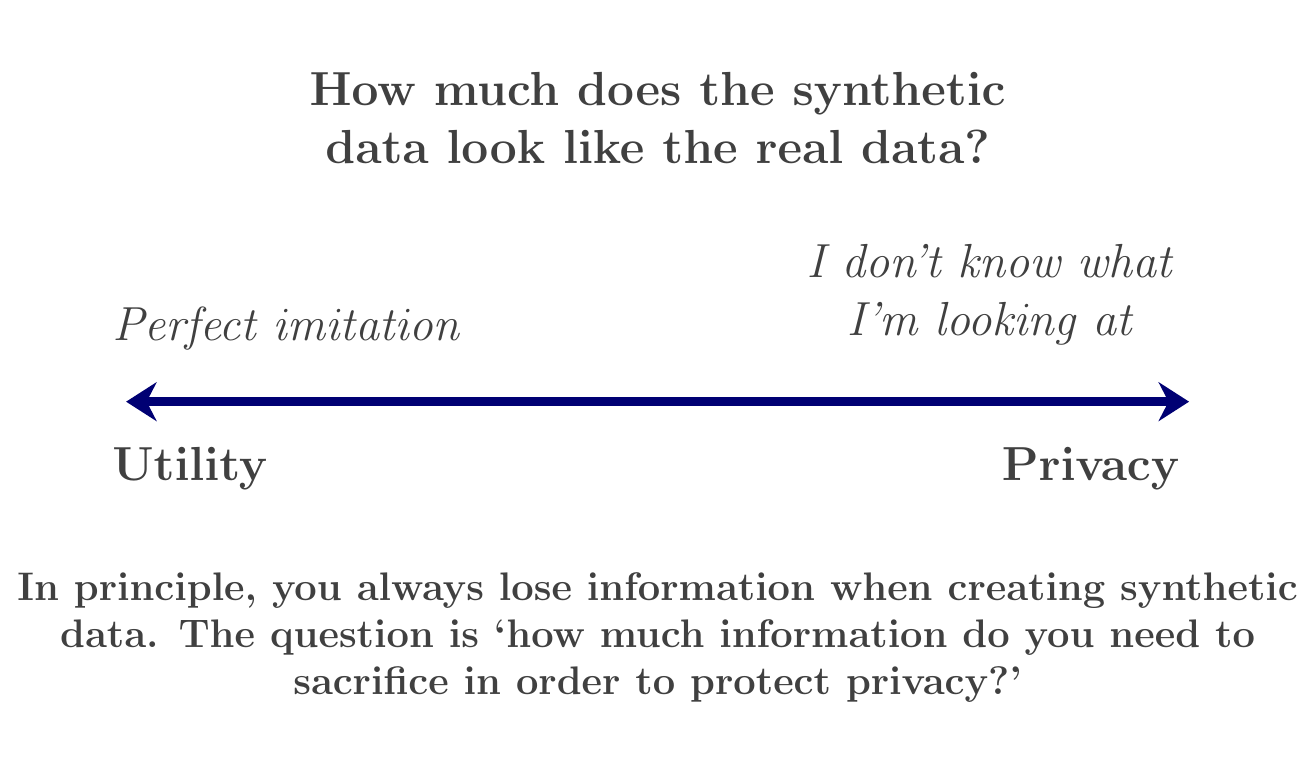
\begin{tikzpicture}[
  x=1cm,
  y=1cm,
  textgray/.style={text=black!75},
  maintext/.style={
    textgray,
    font=\bfseries\fontsize{18}{21}\selectfont,
    align=center
  },
  italictext/.style={
    textgray,
    font=\itshape\fontsize{18}{21}\selectfont,
    align=center
  },
  labeltext/.style={
    textgray,
    font=\bfseries\fontsize{18}{21}\selectfont
  }
]

% Canvas, roughly 16:9
\path[use as bounding box] (0,0) rectangle (16,9);

% Title
\node[maintext] at (8,7.85)
  {How much does the synthetic\\ data look like the real data?};

% Horizontal double arrow
\draw[
  line width=3.2pt,
  color=blue!45!black,
  {Stealth[length=11pt,width=14pt]}-{Stealth[length=11pt,width=14pt]}
] (1.25,4.25) -- (14.75,4.25);

% Upper labels
\node[italictext, anchor=south west] at (0.95,4.78)
  {Perfect imitation};

\node[italictext, anchor=south east] at (14.65,4.85)
  {I don’t know what\\ I’m looking at};

% Lower labels
\node[labeltext, anchor=north west] at (0.95,3.8)
  {Utility};

\node[labeltext, anchor=north east] at (14.75,3.8)
  {Privacy};

% Bottom caption
\node[maintext, font=\bfseries\fontsize{14}{17}\selectfont] at (8,1.25)
  {In principle, you always lose information when creating synthetic\\
   data. The question is ‘how much information do you need to\\
   sacrifice in order to protect privacy?’};

\end{tikzpicture}
\end{document}
